\chapter{Design}
\label{chap:Design}
\emph{``Il semble que la perfection soit atteinte non quand il n'y a plus rien
\`a ajouter, mais quand il n'y a plus rien \`a retrancher.''}

\hfill --- Antoine de Saint-Exup\'ery

\emph{``It can scarcely be denied that the supreme goal of all theory is to
make the irreducible basic elements as simple and as few as possible without
having to surrender the adequate representation of a single datum of
experience.''}

\hfill --- Albert Einstein

\emph{``There are only two kinds of languages: the ones people complain about
and the ones nobody uses.''} \footnote{\emph{Of course, all "there are only
two" quotes have to be taken with a grain of salt.} Bjarne Stroustrup~\cite{stroustrup}}

\hfill --- Bjarne Stroustrup

Programming languages that survived the wilderness of actual usage and
evolution usually suffer from birth or acquired quirks, defects and
idiosyncracies. JavaScript is no exception. In embarking on the journey of
opening it for dynamic instrumentation, we faced the opposing goals of trying
to be compatible with existing programs while keeping the design as simple as
possible. This chapter explains our latest iteration, which runs existing
benchmarks with no modification while providing the flexibility to change the
semantics of object model operations and function calls \textit{while the
program is running}. The runtime environment required to implement the design
can be written in \input{/Users/erick/Recherche/photon-js/perf/loc.txt} lines
of JavaScript code, satisfying our simplicity criteria.

The aim of this chapter is not to provide an exhaustive explanation of how we
handled every idiosyncracy of JavaScript. A reference implementation is
provided for that purpose. Its \textit{raison d'\^etre} is to provide a
high-level overview of the core ideas behind the system, hopefully in a way
that will ease generalization to other languages.

Reification choices, namely the elements of the language we chose to open, are
presented and their particular choice is justified. Then, the message-sending
foundation is explained, both by seeing how the semantic of opened operation
can be expressed on it and how it can be efficiently implemented in JavaScript.
After, an object representation is presented. We believe this representation is
original through its use of proxies that mirror the inheritance chain of the
proxied objects.Finally, a brief compilation example is provided to illustrate
how JavaScript can be compiled to this runtime environment.

\section{Reification choices}

Numerous elements of a programming language can be opened to
user-modifications. A list relevant to JavaScript might include (but not be
limited to):
\begin{itemize}
    \item \textit{Syntax}: How a program is represented (ex: as s-expressions,
    text or graphical tiles)
    \item \textit{Control-flow operators}: The operators modifying the flow of
    control (ex: branching instructions, loops, exceptions, continuations) 
    \item \textit{Environment}: The list of variables accessed by a program and
    their scope (ex: local, global or closure variables)
    \item \textit{Primitive operations}: Operations on primitive values for
    languages that have distinct primitive and object values (ex: \kw{+} in
    JavaScript) 
    \item \textit{Object representation}: How objects are constructed from
    basic elements (ex:Dictionary-based representation, Fixed-memory blocks, etc.)
    \item \textit{Object model operations}: What operations the objects
    support, what behavior they perform and how they affect their
    representation (ex: accessing a property, deleting a property, changing the
    class, etc.)
    \item \textit{Function-calling protocol}: What operations are performed
    before and after a call. (ex: logging type information)
\end{itemize}

Our choice of which elements to reify has been influenced by past empirical
studies choices of data to gather, by the availability of language features
that support the reification and by the optimizations performed by the
underlying runtime. Developments in any of those area will further influence
what elements are interesting, possible and practical to reify, therefore we
urge the reader not to consider this work as the end of the road but instead as
an example of what could be interesting, possible and practical given our
current circumstances. The field is evolving, so should our understanding and
practices.

Given our focus on instrumentating JavaScript, we left out the reification of
the syntax. Our view is that a proper macro system would be ideal, but such a
feature is not necessary to understand what current JavaScript programs are
actually doing. Control-flow operators were left out, mostly for performance
reasons but also because the current version of JavaScript would not allow
their reification easily as a method. Wrapping a block in a function modifies
its environment, potentially changing the \kw{this} value in the block. The
next version of JavaScript introduces an arrow function with a lexical
\kw{this} that will fix this short-coming, so as soon as modern VMs support the
arrow-notation it should be possible to reify the control-flow instructions.
The environment and primitive operations were kept closed for performance
reasons, to ensure fast closure creation, variable access and arithmetic
operations.

The object representation and the object model operations were reified because
a large part of the dynamic instrumentation of JavaScript has targeted the
object model to elucidate the amount of dynamism actually used. This
reification was possible because the primitive operations are extensible
through the \kw{toString} and \kw{valueOf} protocol to support proxy
objects.~\footnote{It was a welcomed feature. It actually made our VM faster by
permitting us to directly use the native primitive operators instead of also
having to reify primitive operation to dispatch to our custom objects.} The
object representation and object model were designed to exploit the host's
inline caches, global function inlining and calling protocol.  

Finally, the function-calling protocol was reified to facilitate the
construction of dynamic call graphs. It was possible because we can globally
transform all functions for support. Our protocol was designed to avoid
reliance on \kw{call} and \kw{apply} native methods and default to the
native calling protocol as long as they are not modified, in the interest of
speed.

\section{Message-sending foundation}
Simplicity is achieved when few abstractions can capture the essence of a whole
class of phenomenons. In our design, the message-sending operation serves to
unify all reified operations around a single mecanism. It facilitates the
achievement of correctness, and arguably, performance, because it allows its
implementation to target the highest performing operations of the underlying
system. It would be unreasonable to expect better performance than a hand-tuned
native implementation~\footnote{However, faster-than-native
speeds might be achieved if the native implementation is suboptimal and performs
worse than a potentially equivalent other native functionality. It is my
conjecture that as systems grow in complexity, such opportunities might be
more common in the future.}. However, this approach might give us a better
performance than equivalent instrumentations that try to optimize every reified
operations independently, without the support of a unified mecanism.

The particular choice of message-sending as a foundation was motivated by its
tried and true application to Smalltalk and Self with success for the obtention
of a dynamic, open and eventually fast implementation. The initial awareness of
the possibility to unify an object model around a message-sending primitive
came from the Open, Extensible Object Models from Piumarta and
Warth~\cite{Piumarta:2008}.

% Open, Dynamic
\subsection{Semantic}

We will now see the chosen semantic for the message-sending operation, in
steps. We will first discuss the basic operation, that closely correspond to a
method call in JavaScript. We will then reify the function call to allow its
redefinition. We will then see how we can reify the memoization operation
performed by inline caches to enable user-supplied functions to specify their
cached behavior, potentially allowing algorithmic improvements in speed. A
message send is always synchronous to another object in the same address space,
which closely micmics the most common usage in recent object-oriented
languages.

To present the message-sending operation, we need to make some assumptions
about the object representation. We will assume, without loss of generality,
that the object representation is itself object-oriented, prototype-based and
that operations to the representation are made by calling methods on
objects.~\footnote{In our particular case, it happens to be the case, as
we will see later in this chapter.} However, the reader should keep in mind
that the message-sending operation is orthogonal to the object representation
chosen. 

We will assume that the representation supports at least 4 methods:
\begin{itemize}
    \item \kw{has(name)} method: returns true if the object has the \kw{name}
    property
    \item \kw{get(name)} method: returns the value of the \kw{name} property on
    this particular object
    \item \kw{call(rcv, ..args)} method: calls the object as a method with the
    \kw{rcv} receiver and \kw{args} arguments and returns its return value
    \item \kw{getPrototype()} method: returns the prototype of an
    object~\footnote{As explained in the conclusion, using the \kw{__proto__}
    property breaks the encapsulation and mixes base-level and meta-level
    information. We therefore prefer to access the prototype through a method
    call. We use it here to advocate this particular usage.}
\end{itemize}

Unless specified, the pseudo-code follows the regular JavaScript semantic. We
will take advantage of the expressivity of the rest and spread operators, bound
to appear in the next revision. For presentation simplicity, primitive values,
missing values and error handling are omitted.

\subsubsection{Basic}

The basic version essentially performs a regular lookup followed by a method
call. The lookup operation is called \kw{bind} to emphasize the
\textit{late-boundness} inherent in a method call, which is the source of
dynamism. This is the semantic of a method call in JavaScript as well:

\jsfile{listings/basic-send.js}

From the point of view of the user program, the \kw{call} operation is opaque
and cannot be modified. When trying to obtain a dynamic call graph, this is
unfortunate, because it forces the rewriting of every call site at compile
time, including method calls, to catch all \textit{call} events.

We can do it dynamically with a slight modification of the semantic of the
operation.

\subsubsection{Augmented function-calling flexibility}

In JavaScript, the \kw{call} method on every function reifies the calling
protocol and allows a program to call into a function at run time, as if it was
done through the direct mecanisms. The exact behavior of a function call should be
the same, whether it is called directly or indirectly. However, there is no
causal relationship between the state of the \kw{call} method and the behavior
of function calls. In other words, redefining the \kw{call} method on
\kw{Function.prototype} does not affect the behavior of call sites.

We can establish this causal relationship with a slight modification of the
send operation:

\jsfile{listings/augmented-send.js}

This semantic allows a particular function to be instrumented, simply be
redefining its call method with proper support. We can also catch all functions
calls, as long as these are mapped to message sends.

Performance \textit{aficionados} might cringe at the idea of adding a level of
indirection to every function call. Before we address performance issue of the
message-sending protocol itself, we first look at a bigger opportunity of
performance gains, namely memoizing the function behavior and see how we can
support it.

\subsubsection{Memoization protocol}

Memoization is usually associated with functional programming and entails
trading space-efficiency for time-efficiency by remembering past return values
of functions with no side-effect. We will use the same definition here although
we will relax the no side-effect constraint by placing the burden of insuring
that memoized functions will always return the same value as if the original
function was called, on the programmer. Whether memoization might break
invariants of the system is left to her to elucidate when writing a particular
memoized function.

This particular functionality became necessary when trying to implement
efficiently the JavaScript object model operations in Photon because they are
reified as methods for openness. It became clear that using inline caches to
memoize their optimized versions was desirable.

The basic idea is to allow a method to inspect its arguments and receiver
before the first call to specialize itself for subsequent calls. The first call
is always performed by calling the original function while all subsequent calls
will be made to the memoized function.

There is an unfortunate interaction between memoization and the reification of
the call protocol. A further refinement specifies that memoization can only
occur if the call method of the function has not been redefined, otherwise it
would change the identity of the function passed to the call method. We simply
need to check if the call method of a function corresponds to the default call
method, in which case the identity of the function is not important, only its
behavior. If it is the case, then, we can store the memoized function in the
cache. Otherwise, we call the original function through its redefined call
method:

\jsfile{listings/memoized-send.js}

This definition has the advantage that one can temporarily redefine the calling
method without penalty after the original method has been restored.

Memoization introduced the idea of a cache for message sends. Caching entails
invalidation if the invariants behind caching are violated. We will see how to
handle that when discussing how to efficiently implement message sending.
Before that, we will see how we can use message sending as a foundation for all
reified operations.

\subsection{Translating reified operations to message-sending}

The following two sections summarize the operations of JavaScript that we
opened by converting them to message sends, according to the semantic presented
precendently.

\subsubsection{Function calls}

Function calls in JavaScript happen in various operations. An explanation of
each occurence as well as their equivalent message send are given in
table~\ref{tb:CallTypes}.

\begin{table}[htb]
\caption{Call types and their equivalent message sends}
\centering

\begin{tabular}{|p{.33\textwidth}|p{.33\textwidth}|p{.33\textwidth}|}
  \hline
  Call Type & Explanation & Equivalent Message Send \\
  \hline \hline
    \tbbox{Global\\} & 
    \tbbox{
        Calling a function whose value is in a global variable. \\
        Ex: \kw{foo()}
    } &
    \tbbox{
        Sending a message on the global object. \\
        Ex: \kw{send(global,"foo")}
    } \\
  \hline
  \tbbox{Local\\} & 
    \tbbox{
        Calling a function in a local variable.  \\
        Ex: \kw{fn()}
    } &
    \tbbox{
        Sending the \kw{call} message to the function.\\
        Ex: \kw{send(fn,"call")}
    } \\
  \hline
  \tbbox{Method\\} & 
    \tbbox{
        Calling an object method. \\
        Ex: \kw{obj.foo()}
    } &
    \tbbox{
        Sending a message to the object.\\
        Ex: \kw{send(obj,"foo")}
    } \\
  \hline
  \tbbox{\kw{apply} or \kw{call}} & 
    \tbbox{
        Calling the \kw{call} or \kw{apply} function method. \\
        Ex: \kw{fn.call()}
    } &
    \tbbox{
        Sending the \kw{call} or \kw{apply} message.\\
        Ex: \kw{send(fn,"call")}
    } \\
  \hline
\end{tabular}

\label{tb:CallTypes}
\end{table}


\subsubsection{Object model operations}

An explanation of each opened object model operation as well as their
equivalent message send are given in table~\ref{tb:ObjectModelOperations}.

\begin{table}[htb]
\caption{Object model operations and their equivalent message sends}
\centering

\begin{tabular}{|p{.33\textwidth}|p{.33\textwidth}|p{.33\textwidth}|}
  \hline
  Object Model Operation & Explanation & Equivalent Message Send \\
  \hline \hline
  \tbbox{Property access} & 
    \tbbox{
        Retrieving the value of a property that might exist or not.\\
        Ex: \kw{obj.foo}  
    } &
    \tbbox{
        Sending the \kw{__get__} message.\\
        Ex: \kw{send(obj,"__get__","foo")}
    } \\
  \hline
  \tbbox{Property assignation} & 
    \tbbox{
        Creating or updating a property.\\
        Ex: \kw{obj.foo=42} 
    } &
    \tbbox{
        Sending the \kw{__set__} message.\\
        Ex: \kw{send(obj,"__set__","foo",42)}
    } \\
  \hline
  \tbbox{Property deletion} &
    \tbbox{
        Deleting a property that might exist or not.\\
        Ex: \kw{delete obj.foo}
    } &
    \tbbox{
        Sending the \kw{__delete__} message. Ex:\\
        \kw{send(obj,"__delete__","foo")}
    } \\
  \hline
  \tbbox{Object litteral creation} & 
    \tbbox{
        Creating an object in-place.\\
        Ex: \kw{\{foo:42\}} 
    } &
    \tbbox{
        Sending the \kw{__new__} message.\\
        Ex: \kw{send(\{foo:42\}, "__new__")}
    } \\
  \hline
  \tbbox{Constructor creation} & 
    \tbbox{
        Creating an object with \kw{new}. \\
        Ex: \kw{new Fun()}
    } &
    \tbbox{
        Sending the \kw{__ctor__} message.\\
        Ex: \kw{send(Fun, "__ctor__")}
    } \\
  \hline
\end{tabular}

\label{tb:ObjectModelOperations}
\end{table}

\subsection{Efficient implementation}
Now that the semantic and mapping have been established, we will address the
biggest hurdle that might prevent an approach based on a unified message
sending foundation to be used, namely performance.

The core insight behind our implementation comes from seeing global function
calls both as an optimized calling mecanism and as a dynamically specializable
operation. They provide the same ability as code patching in assembly. On
the current version of V8, when the number of arguments expected matches the
number of arguments supplied, it opens the possibility of inlining the function
at the call site. If later the global function is redefined, the call site will
be deoptimized transparently. It is a really powerful mecanism because much of
the complexity of run-time specialization is performed by the underlying host.
We can simply piggy back on those optimizations.

Let's start with an example. Given the aforementioned semantic of message
sending, sending the message \kw{msg} to an object \kw{obj} inside a \kw{foo}
function can be written this way:

\jsfile{listings/send-example.js}

The \kw{send} function is a global function. We can replace it with another
global function that is garanteed to be unique, so it can be uniquely
identified with the call site. In addition to the message to be sent, we can
pass it a unique identifier that will be used to find the corresponding global
function name, for later specialization of the call site:

\jsfile{listings/inline-cache-example.js}

Notice how the \kw{initState} function follows the same calling convention as
the \kw{send} function. As we will see later, it is also the same calling
conventions used for our function call protocol. Notice also that
\kw{dataCache0} is an array, which means that the different states of the cache
can use the array to store additional information.

After an initial execution, the second time around, the cache will hold an
optimized version of the operation. From now on, we will use the object
representation we defined previously with a slight difference: we will assume
the \kw{get} operation performs an implicit lookup through its prototype chain,
as previously we stated that it would only lookup on the current object.
Given this new definition, the cache state might be equivalent to:

\jsfile{listings/inline-cache-optimized-example.js}

Appart from the indirection of the global function call, this example is
optimal with regard to the object representation definition we have. If the
underlying runtime choose to inline the global function, the cost of the
indirection will be effectively eliminated.

\subsubsection{Cache states and transitions}

We can build on the previous insight by precisely defining the behaviors of the
inline caches and the conditions that trigger those behaviors. There are
various ways to do it with different performance and flexibility profiles. We
have not exhaustively explored the possibilities, therefore there might be
interesting configurations yet to be uncovered. Nonetheless, we still found a
simple arrangement that allows reified operations to be specialized to their
call sites with a small memory overhead in terms of tracking run-time
invariants.  An enthousiastic reader should read the following not as the final
word on the matter but as a point of departure, as we believe there are other
interesting configurations to be found.

We use a state machine formalism to present the different behaviors associated
with inline caches and the triggers that are responsible for the transitions
between those behaviors. In our formalism, due to the nature of synchronous
message sends, a state transition occurs before the event has been fully
processed. However the processing of the event is not influenced by it.  

To simplify invariants tracking, we decided to always perform lookups for
regular method calls. By making the lookup operation as close as possible to
the native operation of JavaScript, it allows the underlying VM to optimize it.
In our design, the idea is to delegate the regular method call to the object
representation. The other important operation was to allow specialization of
object model operations, which is critical for speed. This is done by memoizing
a specialized version in the inline cache. We therefore ended up with two
states in addition to the initial state of the cache, as explained in
table~\ref{tb:CacheStates}.

\begin{table}[htb]
\caption{Cache states}
\centering

\begin{tabular}{|p{.33\textwidth}|p{.33\textwidth}|}
  \hline
  Cache states & Explanation \\
  \hline \hline
  \tbbox{Initial State} & 
    \tbbox{
        Perform a regular send.
    } \\
  \hline
  \tbbox{Regular method call} & 
    \tbbox{
        Lookup method then call.
    } \\
  \hline
  \tbbox{Memoized method call} & 
    \tbbox{
        Method specific behavior. The memoized method is responsible for
        maintaining invariants.
    } \\
  \hline
\end{tabular}

\label{tb:CacheStates}
\end{table}


Transitions between states happen on message send and object model operation
events.  An insight was to realize that we could under-approximate the tracking
of invariants and invalidate conservatively more caches than what would
minimally be required. As long as the operations triggering the invalidation of
caches are infrequent, the performance impact should be minimal. We therefore
track method values cached in memoized states by name without consideration of
the receiver object. If a method with the same name is updated on any object,
all caches with a given message name will be invalidated. Also, if the
\kw{call} method on the \kw{Function.prototype} object or any method with the
\kw{__memoize__} name is updated, \textit{all} caches will be invalidated. This
way, we can only track caches associated with names. The upper bound on memory
usage for tracking information is proportional to the number of cache sites.

There is no state associated with a redefined \kw{call} method. In that
particular case, all caches will stay in the initial state and a regular
message send will be performed (and not cached). Figure~\ref{fig:CacheStates}
summarizes those elements in a state diagram. A more detailed explanation of
every event and transition conditions are given in table~\ref{tb:CacheEvents}
and table~\ref{tb:CacheTransitionConditions}.

\begin{figure}[htb]
\begin{center}
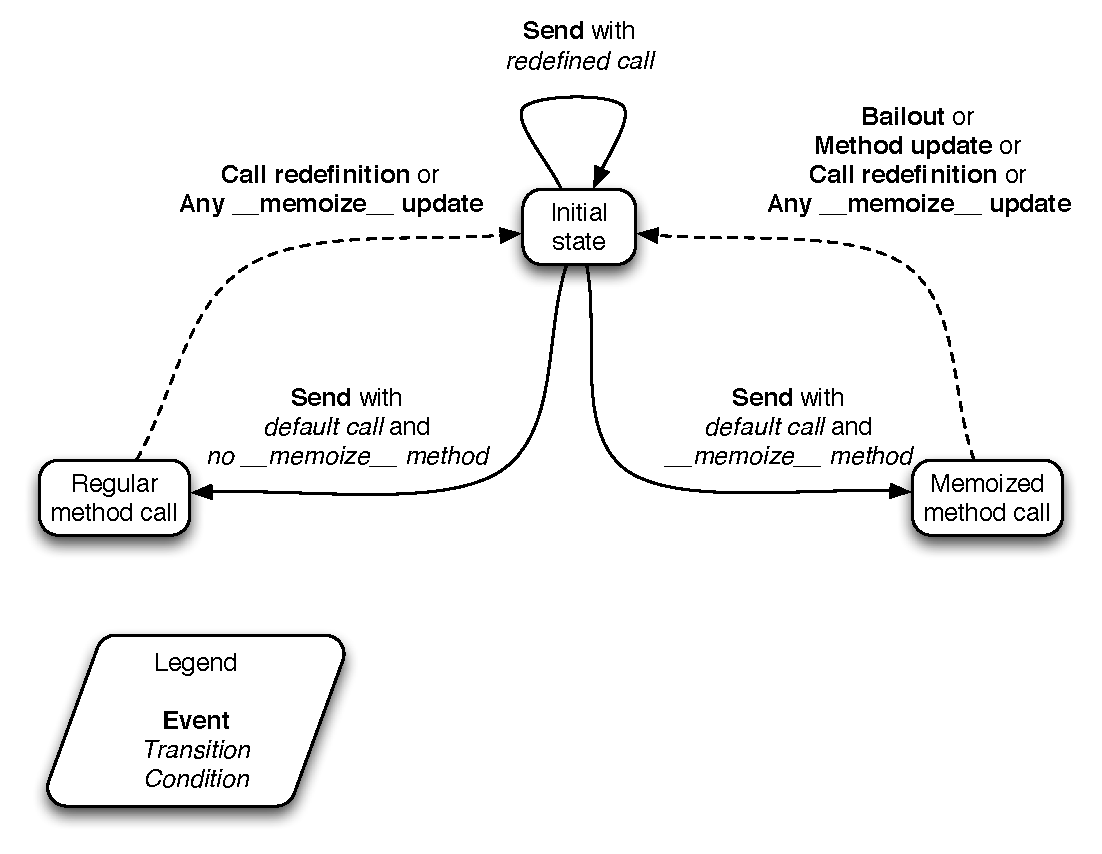
\includegraphics[width=\textwidth]{figures/cacheStates}
\caption{\label{fig:CacheStates} Cache States and Transitions}
\end{center}
\end{figure}

\begin{table}[htb]
\caption{Cache Events}
\centering

\begin{tabular}{|p{.33\textwidth}|p{.33\textwidth}|}
  \hline
  Cache Events & Explanation \\
  \hline \hline
  \tbbox{Send} & 
    \tbbox{
    A message is sent to a receiver object.
    } \\
  \hline
  \tbbox{Call redefinition} & 
    \tbbox{
    The \kw{call} method on \kw{Function.prototype} is redefined.
    } \\
  \hline
  \tbbox{Any memoized redefinition} & 
    \tbbox{
    Any \kw{__memoize__} method is being redefined.
    } \\
  \hline
  \tbbox{Bailout} & 
    \tbbox{
    A run-time invariant has been violated.
    } \\
  \hline
  \tbbox{Method redefinition} & 
    \tbbox{
    An object with a method with the same name has his method being updated.
    } \\
  \hline
\end{tabular}

\label{tb:CacheEvents}
\end{table}

\begin{table}[htb]
\caption{Cache Transition Conditions}
\centering

\begin{tabular}{|p{.33\textwidth}|p{.33\textwidth}|}
  \hline
  Cache Transition Condition & Explanation \\
  \hline \hline
  \tbbox{Default call} & 
    \tbbox{
    \kw{Function.prototype call} method is the same as the one initially supplied.
    } \\
  \hline
  \tbbox{Redefined call} & 
    \tbbox{
    \kw{Function.prototype call} method is different than the one initially supplied.     
    } \\
  \hline
  \tbbox{No \kw{__memoize__} method} & 
    \tbbox{
    No method named \kw{__memoize__} has been found on the method to be called.
    } \\
  \hline
  \tbbox{\kw{__memoize__} method} & 
    \tbbox{
    A method named \kw{__memoize__} has been found on the method to be called.
    } \\
  \hline
\end{tabular}

\label{tb:CacheTransitionConditions}
\end{table}

The initial inspiration for optimizing sends with global functions that would
change during execution was drawn from the lazy function definition pattern as
explained by Peter Michaux, in which after the initial setup performed by a
function, a new function without the initialization code can replace the
original function to provide an efficient
operation~\cite{michaux:LazyFunctionDefinitionPattern}. We believe this is the
first time this pattern is used as an inline cache in the litterature.

For simplicity reasons, we did not try to aim for robustness in addition to
flexibility and performance. It is therefore possible to break the system by
supplying a memoized method that does not correctly maintain invariants. We
decided to aim for maximum flexibility with a simple mecanism that could be
used to specialize object model operations. The responsibility of supplying a
correct method is left on the programmer. That being said, we believe it should
be possible to further constrain this flexibility for robutness, within the
same framework.

\section{Object Representation}
% Performance, Extensible
\subsection{Prototype-based}
\subsection{Proxy}
\subsection{Containers}
\subsection{Optimization opportunities}
\subsubsection{Specialized operations}
\subsubsection{Specialized arguments length}

\section{Function-calling protocol}



\section{Compilation}
\subsection{Examples}

